\documentclass[12pt,letterpaper]{article}
\usepackage[dvipdfm,top=1in, bottom=1in, left=.85in, right=0.850in]{geometry}
\usepackage[T1]{fontenc}
\usepackage[latin1]{inputenc}
\usepackage{palatino,courier}
\usepackage[reqno]{amsmath}
\usepackage{amsthm}
\usepackage{amsfonts,amssymb}
\usepackage[mathscr]{euscript}
\usepackage[all]{xy}
\usepackage{stmaryrd}
\usepackage{proof}
\usepackage{fancyhdr}
\usepackage{varioref}
\usepackage{xspace}
\usepackage{graphicx}
\usepackage[colorlinks=true,letterpaper=true]{hyperref}
\CompileMatrices
 
\title{LQPL - Design}
\pagestyle{fancy}
\headheight15pt
\lfoot{Giles}
\cfoot{\thepage}
\rfoot{\emph{In development}}
\rhead{\today}
\lhead{\textbf{LQPL Design}}
\chead{}
\author{Brett Gordon Giles}
\begin{document}
\begin{table}[htdp]
\caption{Commands for UI to Emulator}
\begin{center}
\begin{tabular}{|p{1.5in}|p{2.1in}|p{2.1in}|}
\hline
Command&Effect &Returns \\ \hline
Step $n$, ($n\ge 1$) & execute $n$ instructions& Nothing \\ \hline
Go & execute until done &Nothing\\ \hline
GetQstack $n$ $m$ & None & Return structured tree down to depth $n$ using $m$-th iteration of infinite list of stacks.\\ \hline
GetCstack $m$ & None &Classical stack using $m$-th iteration of infinite list of stacks. \\ \hline
GetDump $n$ $m$ & None & Structured version of dump, using $m$ for infinite list of stacks, $n$ for
depth of individual QStacks. \\ \hline
Reset & Sets stacks to empty, Qstack to 0/1, code pointer to entry point & Nothing\\ \hline
Load \emph{code} & resets machine and loads code & Nothing \\
\hline
\end{tabular}
\end{center}
\label{default}
\end{table}%
\begin{figure}[htbp]
\begin{center}
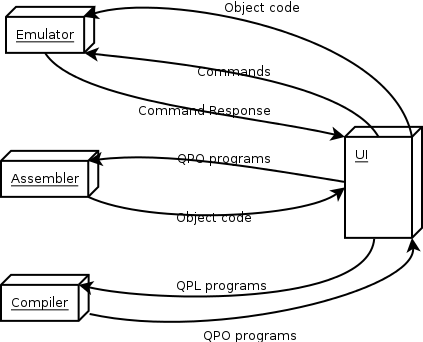
\includegraphics{FourModules.png}
\caption{Modules}
\label{default}
\end{center}
\end{figure}


\end{document}